\section{Integration Tests}

Integration tests come next to ensure each unit functions
correctly when interacting with other units in the
application.

In contrast to unit tests, integration tests in
\projectname{} ensure the business features are implemented
as designed; this is focussed mainly on the various
constraints and preconditions when
\glsdisp{clock-in}{clocking in}/ \glsdisp{clock-out}{out}
and confirming another employee.

\begin{figure}[h]
  \centering
  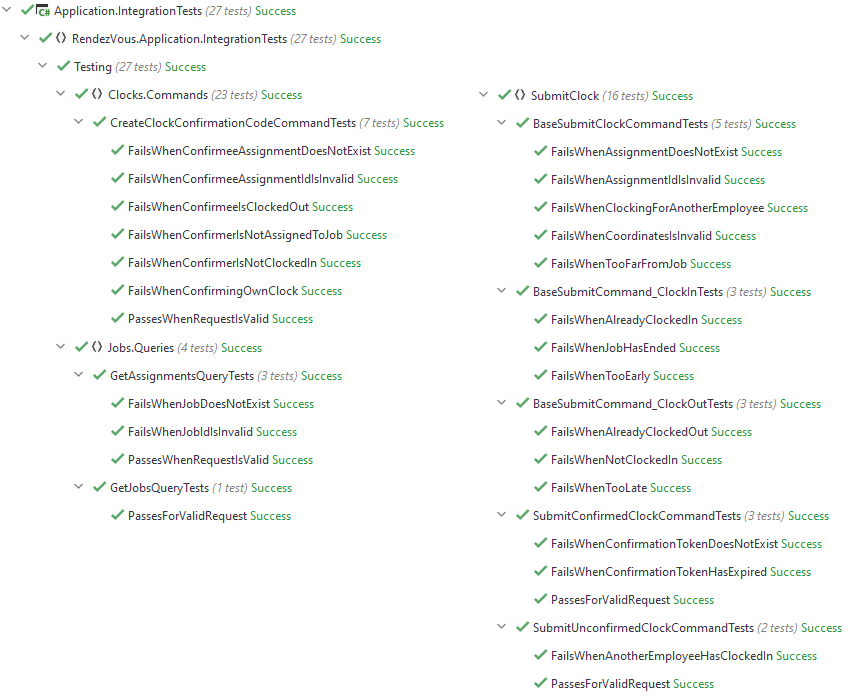
\includegraphics[width=0.9\linewidth]{07 testing/assets/integration/test runner.png}
  \caption{Integration Tests in the API}
  \label{fig:integrationTestRunner}
\end{figure}

Figure \ref{fig:integrationTestRunner} shows the difference
in testing simple simple and complex functionality.
Querying for jobs requires only one file, whereas the rules
for clocking require many more tests spread across multiple
files.

